\documentclass{article}


\usepackage[utf8]{inputenc} % allow utf-8 input
\usepackage[T1]{fontenc}    % use 8-bit T1 fonts
\usepackage{hyperref}       % hyperlinks
\usepackage{url}            % simple URL typesetting
\usepackage{booktabs}       % professional-quality tables
\usepackage{amsfonts}       % blackboard math symbols
\usepackage{nicefrac}       % compact symbols for 1/2, etc.
\usepackage{microtype}
\usepackage{amsmath}      % microtypography
\usepackage{bm}
\usepackage{graphicx}
\usepackage{verbatim}
\usepackage{wrapfig}
\usepackage[font=small]{caption}
\usepackage{enumitem}
\usepackage{amsmath}
%\usepackage{floatrow}

%\addtolength{\belowcaptionskip}{-20pt}

\title{test}

\begin{document}

\maketitle

%\begin{abstract}
%  TODO
%\end{abstract}

%\vspace*{-7em}

\section{Introduction}

dp:
pros: hard-constraint satisfied by design (as reflected by valid recursion steps);
models distribution
cons: efficient dp recursion based on nesting assumption, cannot model pseudoknot;
additive energy terms, hard-coded.

scfg & extension:
pros: constraints;
models distribution
trainable param
cons: efficient dp recursion based on nesting assumption, cannot model pseudoknot


todo: plot explaining dp & scfg approaches

nn:
pros: expressive, can be trained on lots of data;
cons: too many parameters, risk of overfitting if trained on dataset not diverse enough;
hard constraints cannot be captured by default
(some work using optimization as unrolled rnn, but no guarantee it'll converge,
and even if it converges there's guarantee the output satisfies the constraints,
since the original discrete variables need to be relaxed in order to run through the optimization nn,
so we're no longer operating in discrete space);
does not model distribution

todo: plot explaining nn approaches


In this work we are aiming at developing a model that makes use of the expressiveness of deep nn
while respecting the hard constraints.

This report covers the following sections:

- predictive problem formulation

- we review the commonly used data representation for rna ss

- we propose an alternative way to represent/parameterized the ss

- under the alternative parametrization, we propose a 2-stage model,
which satisfies the biological hard constraints by design

- describe stage 1 model: data, training & result.


- ideas for stage2


\subsection{Problem formulation}

Given an RNA sequence of length $L$, we are interested in all possible secondary structures.
%There are three common ways to represent a specific RNA secondary structure:
To represent a specific secondary structure, there are three commonly used conventions:
(1) undirected graph, where each node is a base in the sequence, and each edge represents base pairing.
(2) upper triangular matrix (excluding the diagonal)
of size $L \times L$ with binary values, where a value of $1$ at $(i, j)$ represents
base pairing between sequence position $i$ and $j$, and $0$ represents no base paring.
(3) dot-bracket notation of length $L$ where unpaired bases are denoted as dots,
    and paired bases are represented as left and right brackets.
%When pseudoknot is present, different styles of bracket needs to be used to represent nested structures.


As an example, for a short RNA sequence GUUGUGAAAU, one possible structure it can take on

consists of a stem and a loop, as seen in Fig \ref{fig:rna_ss_binary_mat}(a), represented by an undirected graph.
Such structure can also be represented by a $10 \times 10$ upper triangular matrix with all $0$'s,
except for positions
%$y_{1, 10}, y_{2, 9}$ and $y_{3, 8}$,
$(1, 10), (2, 9)$ and $(3, 8)$,
all being $1$, as shown in Fig \ref{fig:rna_ss_binary_mat}(b).
This contiguous stretch of $1$'s along the diagonal corresponds to the stem formed by the three base pairs: G-U, U-A and U-A.
The equivalent dot-bracket notation is shown in Fig \ref{fig:rna_ss_binary_mat}(c), where the stem is represented
by three pairs of left-right brackets.
%(TODO define x and y first)



\subsection{Structural components}

Just as sequence motif is defined in the linear sequence space,
a similar notion of 'structural motif' also exists.
A commonly adopted way is to break down structure into the following components:

\begin{itemize}
    \item stem: todo
    \item hairpin loop: todo
    \item internal loop: todo
    \item bulge: todo
    \item external loop: todo
    \item multibranch loop: todo
    \item pseudoknot: todo
\end{itemize}

Such structural motifs can be easily identified on the graph representation of a structure,
as shown in Fig \ref{fig:structural_motif_graph}, where we only annotated one instance for each structural motif class for clarity.
(todo add a minimal example for pseudoknot)

\begin{figure}[h]
    \centering
    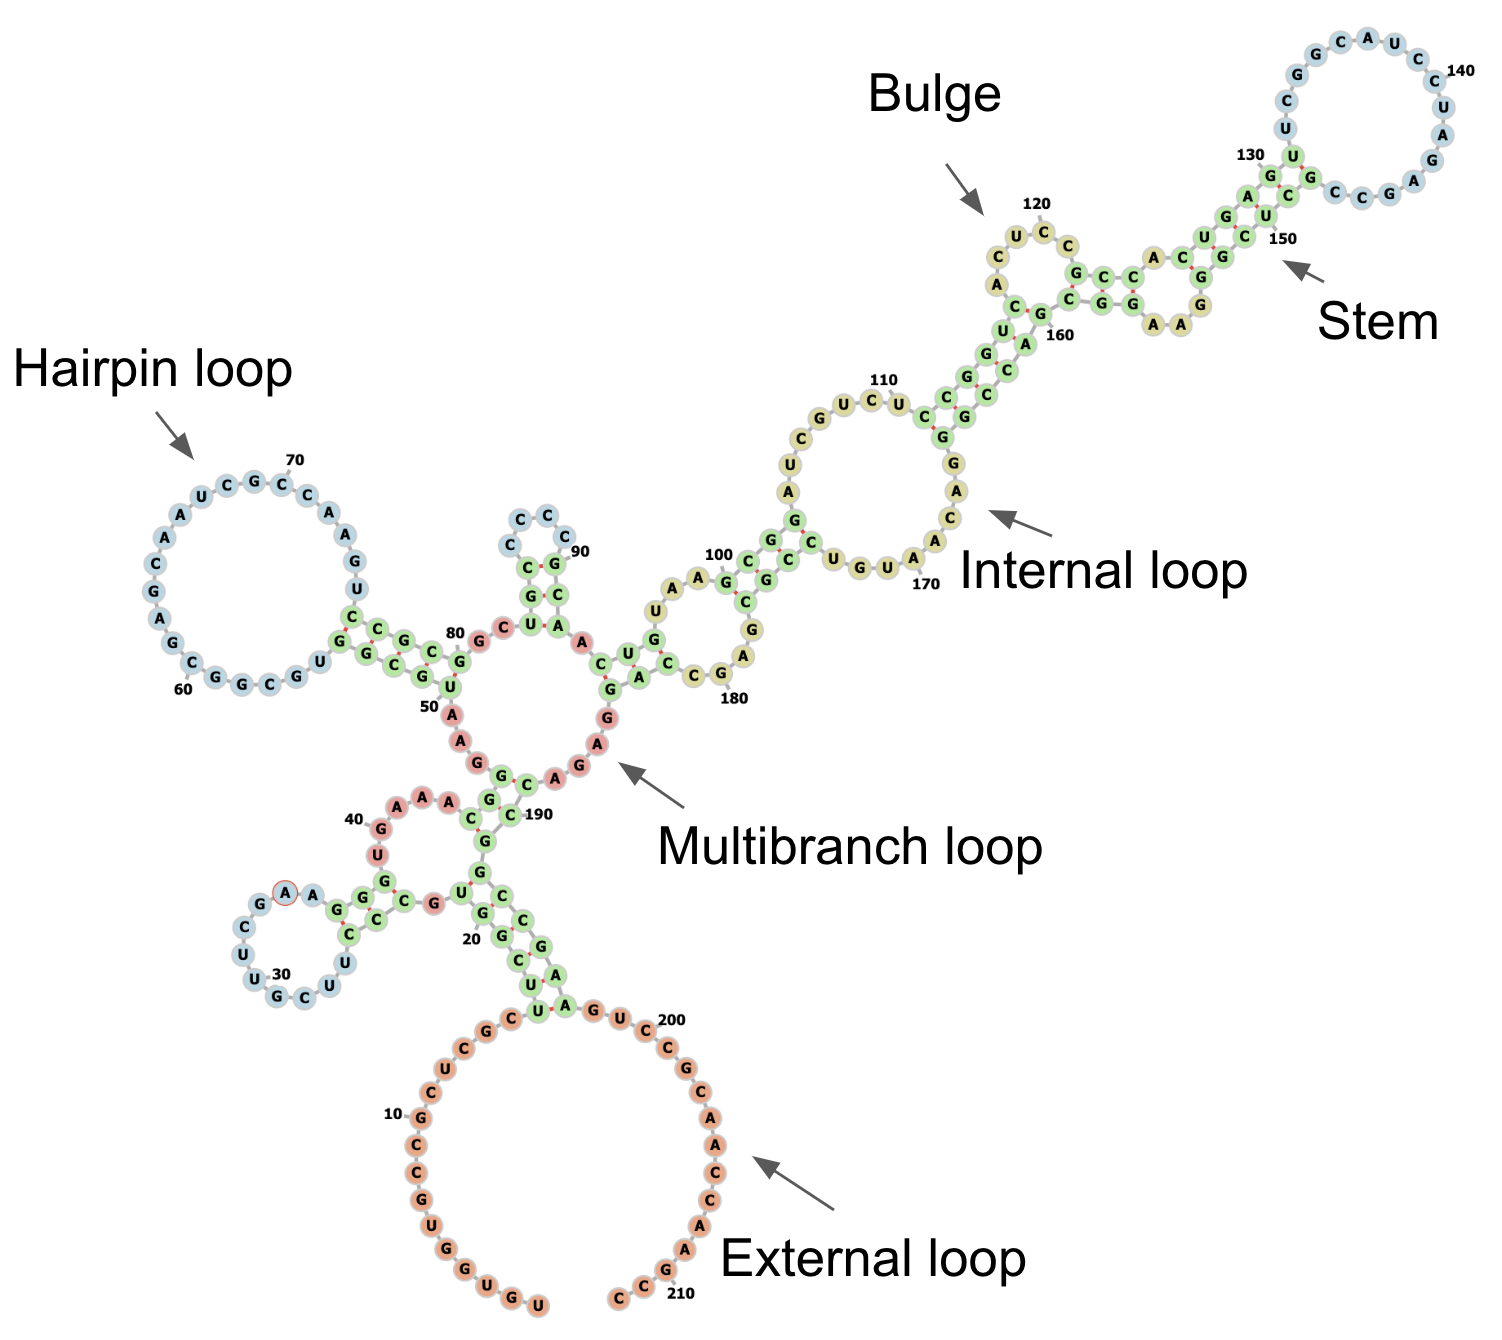
\includegraphics[width=0.8\textwidth]{plot/structural_motif_graph.png}
    \caption{TODO}
    \label{fig:structural_motif_graph}
    \centering
\end{figure}


In this work, we distinguish structural motifs that are 'local' and 'non-local',
where local-ness is defined w.r.t. the 2D matrix representation of the structure.
To illustrate this idea, we plot the 2D matrix corresponding to the above structure,
as shown in Fig \ref{fig:structural_motif_2d_matrix}(a).
For each type of structural motif, if it can be fully represented by the interaction between
two (contiguous) substrings of the original sequence, it is considered a 'local' structure,
and can be fully identified by a bouning box on 2D matrix representation.
Note that interaction does not necessarily mean the substrings bind to each other.
On the other hand, certain structure motifs can only be represented by interaction between
more than two (contiguous) substrings of the original sequence, then it is a non-local structure.

\begin{figure}[h]
    \centering
    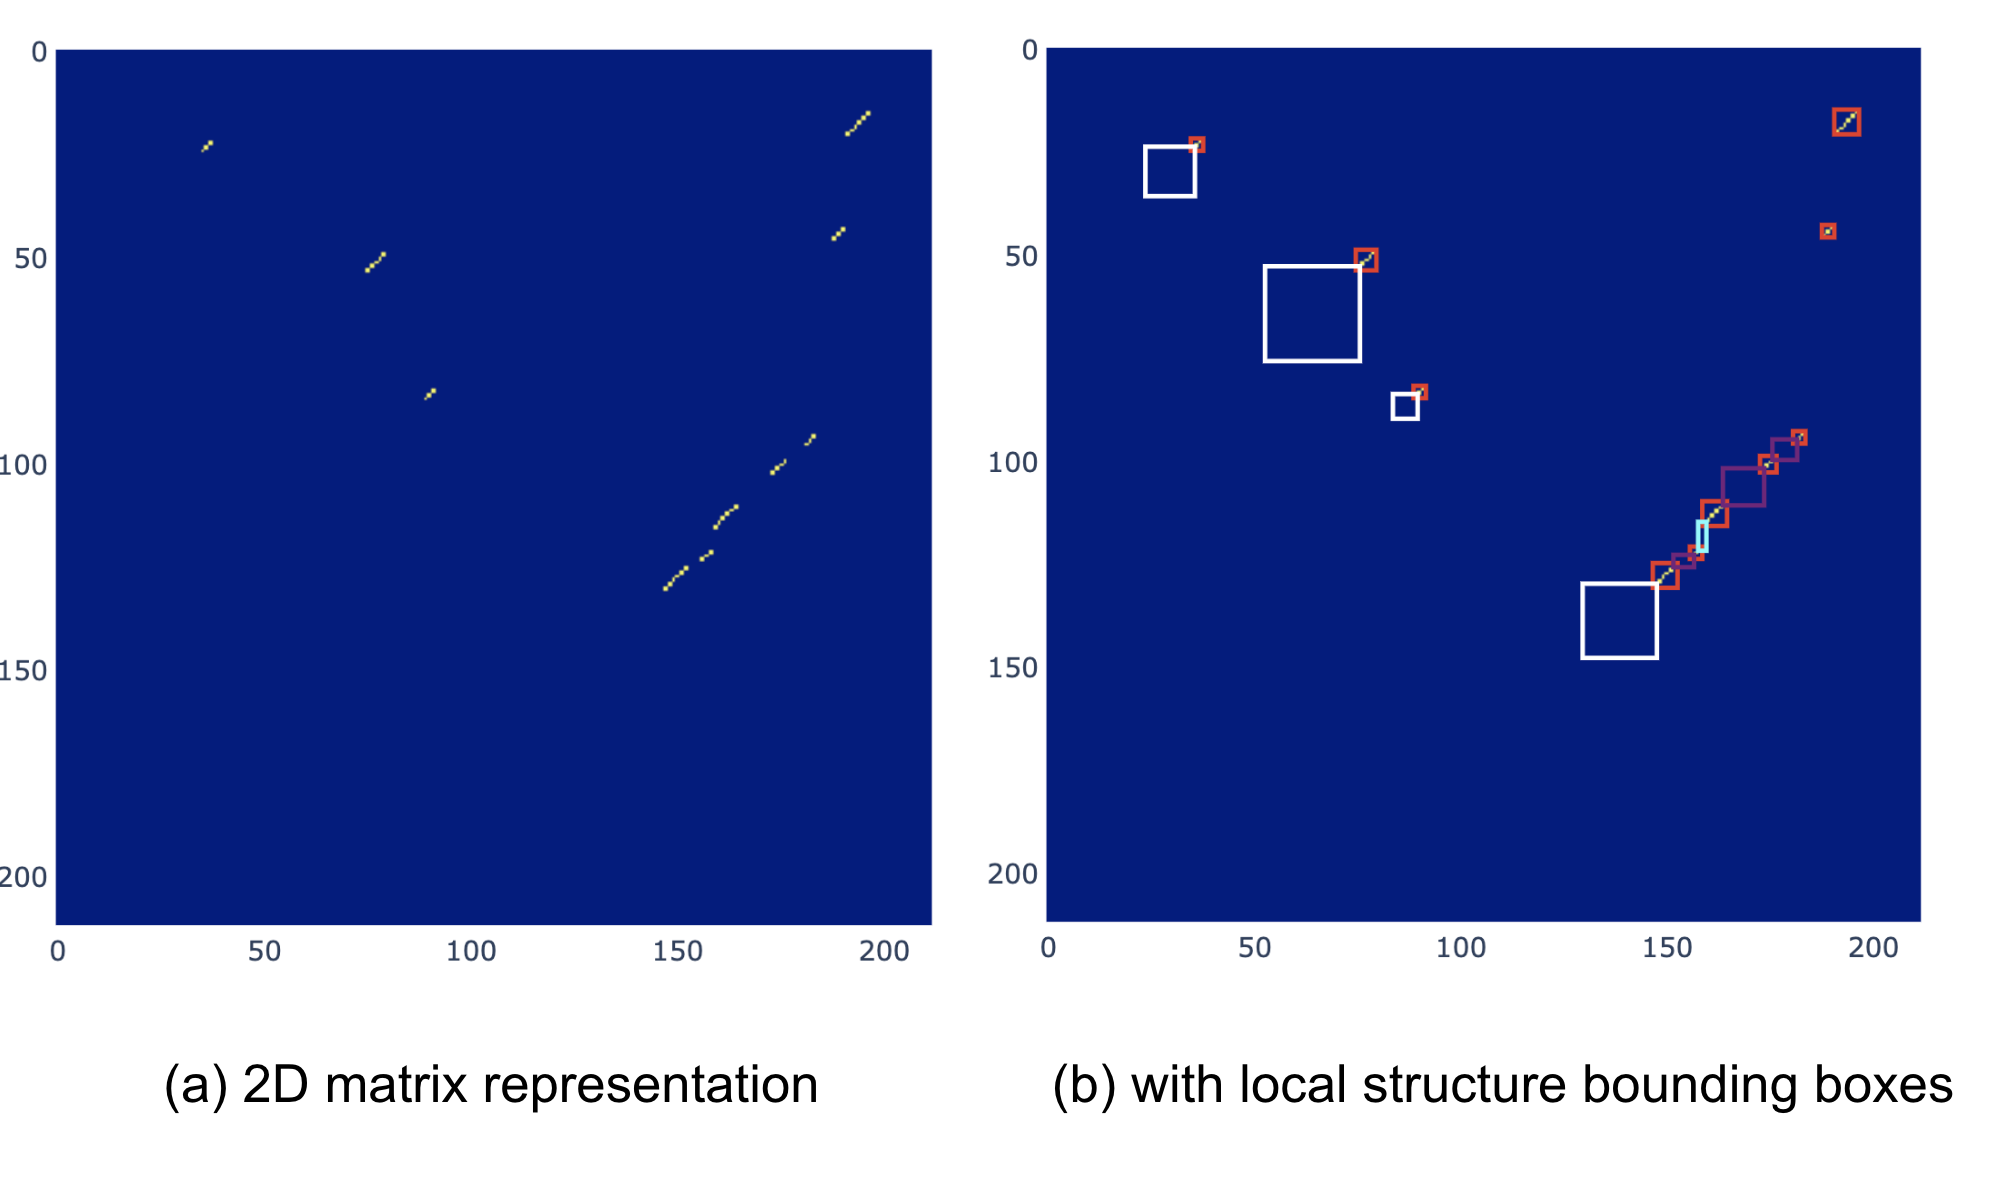
\includegraphics[width=\textwidth]{plot/structural_motif_2d_matrix.png}
    \caption{TODO}
    \label{fig:structural_motif_2d_matrix}
    \centering
\end{figure}





Using the above defined, we drew all the local structure bounding boxes,
as shown in Fig \ref{fig:structural_motif_2d_matrix}(b).


\begin{figure}[h]
    \centering
    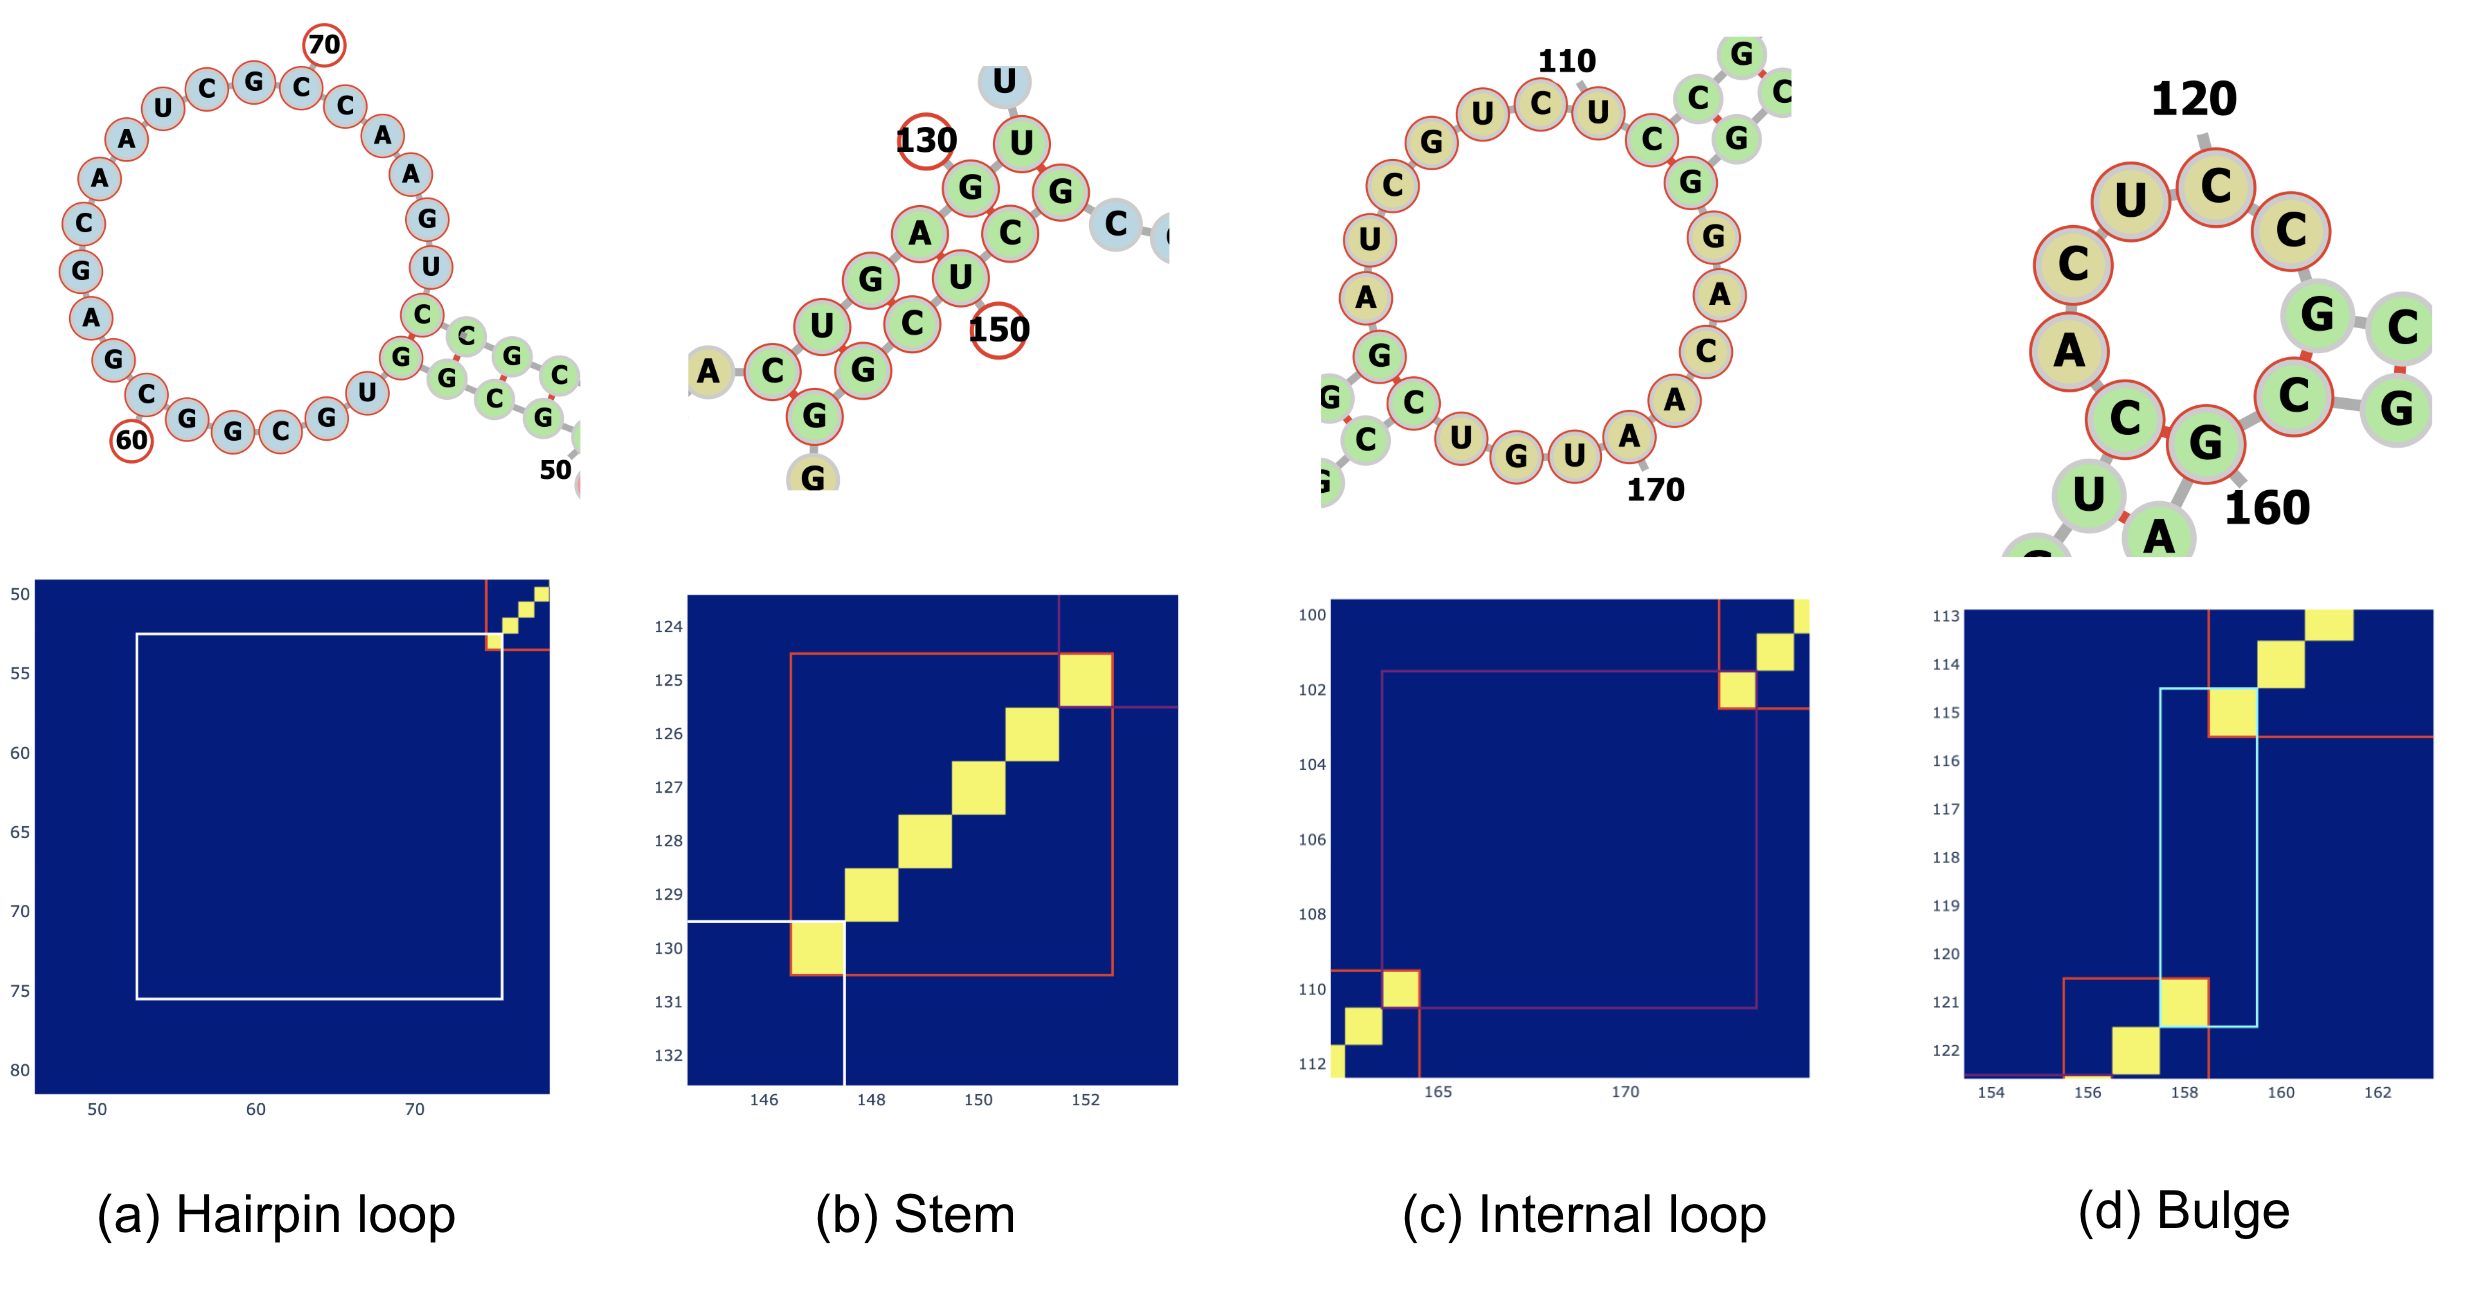
\includegraphics[width=\textwidth]{plot/local_bounding_box_examples.png}
    \caption{TODO}
    \label{fig:local_bounding_box_examples}
    \centering
\end{figure}


To precisely define what constitutes each type of local structure,
we zoom in to each one annotated in Fig \ref{fig:structural_motif_graph},
and compare it with the corresponding zoomed-in 2D matrix, as shown in
Fig \ref{fig:local_bounding_box_examples}.
As we can see:

todo


Formal definition and minimal example




no need for additional parameters







\subsection{Related work}



\section{Method}



\subsection{Architecture}


\subsection{Training}



\subsection{Inference} \label{sec:inference}



\section{Result}

\subsection{Test set performance}


\subsection{Structures with pesudoknot}


\bibliographystyle{unsrt}
\bibliography{report}

%Speed consideration: implement split architecture, only need one forward pass for up to the last layer,
%then run last layer (triangular convolution) for $L-1$ times.
%
%
%Case study:
%
%TODO compare with RNAfold performance


\end{document}
